\documentclass[a4paper, UTF-8]{article}
\usepackage{algorithm}
\usepackage{algpseudocode}
\usepackage{amsmath}
\usepackage{amsfonts}
\usepackage{amsthm}
\usepackage{tikz}
\usetikzlibrary{automata, positioning, arrows, trees}
\usepackage[utf8]{inputenc} % allow utf-8 input
\usepackage[T1]{fontenc}    % use 8-bit T1 fonts
\usepackage{hyperref}       % hyperlinks
\usepackage{url}            % simple URL typesetting
\usepackage{booktabs}       % professional-quality tables
\usepackage{amsfonts}       % blackboard math symbols
\usepackage{nicefrac}       % compact symbols for 1/2, etc.
\usepackage{microtype}      % microtypography
\usepackage{xcolor}         % colors

\theoremstyle{plain}
\newtheorem{theorem}{\indent Theorem}[section]
\newtheorem{lemma}[theorem]{\indent Lemma}
\newtheorem{assumption}{\indent Assumption}[section]
\newtheorem{note}[theorem]{\indent Notation}
\newtheorem{proposition}[theorem]{\indent Proposition}
\newtheorem{corollary}[theorem]{\indent Corollary}
\newtheorem{definition}{\indent Definition}[section]
\newtheorem{example}{\indent Example}[section]
\newtheorem{remark}{\indent Remark}[section]
\newenvironment{solution}{\begin{proof}[\indent\bf Solution]}{\end{proof}}
\renewcommand{\proofname}{\indent\bf Proof}

\begin{document}

\title{\bf{Lab5 Answers}}

\author{Yanqiao Chen*\\ 
  Department of Computer Science and Engineering\\
  Southern University of Science and Technology\\
  \texttt{12412115@mail.sustech.edu.cn}
  }

\maketitle

\section{Question 1} 

\subsection*{a) $a$}
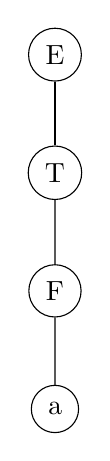
\begin{tikzpicture}[
  level 1/.style={sibling distance=2cm},
  every node/.style={circle, draw, minimum size=6mm}
]
\node {E}
  child { node {T}
    child { node {F}
      child { node {a} }
    }
  };
\end{tikzpicture}

\subsection*{b) $a+a$}
\begin{tikzpicture}[
  level 1/.style={sibling distance=3cm},
  level 2/.style={sibling distance=1.5cm},
  every node/.style={circle, draw, minimum size=6mm}
]
\node {E}
  child { node {E}
    child { node {T}
      child { node {F}
        child { node {a} }
      }
    }
  }
  child { node[rectangle, inner sep=2pt] {$+$} }
  child { node {T}
    child { node {F}
      child { node {a} }
    }
  };
\end{tikzpicture}

\subsection*{c) $a+a+a$ ($(a+a)+a$)}
\begin{tikzpicture}[
  level 1/.style={sibling distance=4.5cm},
  level 2/.style={sibling distance=2cm},
  level 3/.style={sibling distance=1.2cm},
  every node/.style={circle, draw, minimum size=6mm}
]
\node {E}
  child { node {E}
    child { node {E}
      child { node {T}
        child { node {F}
          child { node {a} }
        }
      }
    }
    child { node[rectangle, inner sep=2pt] {$+$} }
    child { node {T}
      child { node {F}
        child { node {a} }
      }
    }
  }
  child { node[rectangle, inner sep=2pt] {$+$} }
  child { node {T}
    child { node {F}
      child { node {a} }
    }
  };
\end{tikzpicture}

\subsection*{d) $((a))$}
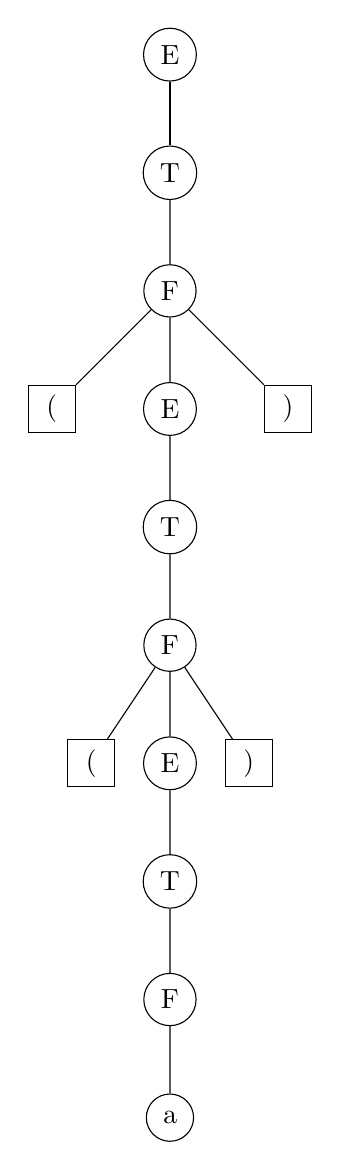
\begin{tikzpicture}[
  level 1/.style={sibling distance=2.5cm},
  level 2/.style={sibling distance=2cm},
  level 3/.style={sibling distance=1.5cm},
  level 4/.style={sibling distance=1cm},
  every node/.style={circle, draw, minimum size=6mm}
]
\node {E}
  child { node {T}
    child { node {F}
      child { node[rectangle, inner sep=2pt] {(} }
      child { node {E}
        child { node {T}
          child { node {F}
            child { node[rectangle, inner sep=2pt] {(} }
            child { node {E}
              child { node {T}
                child { node {F}
                  child { node {a} }
                }
              }
            }
            child { node[rectangle, inner sep=2pt] {)} }
          }
        }
      }
      child { node[rectangle, inner sep=2pt] {)} }
    }
  };
\end{tikzpicture}

\section{Question 2} 

\begin{itemize} 
    \item [a.] $R, X, S, T$ 
    \item [b.] $a, b$ 
    \item [c.] $R$ 
    \item [d.] $ab$, $ba$, $aab$ 
    \item [e.] $aaaa$, $bbbb$, $aaaaaa$
    \item [f.] False. 
    \item [g.] True. 
    \item [h.] False. 
    \item [i.] True.  
    \item [j.] True. 
    \item [k.] False.
    \item [l.] True.
    \item [m.] True. 
    \item [n.] False.
    \item [o.] All non-palindromic strings over \{a,b\} that have at least one mismatched symmetric pair (a,b) or (b,a).
\end{itemize}

\section{Question 3} 

\subsection{a)} 

\begin{align*}
S \to R1R1R1R \\
R \to 0R \mid 1R \mid \epsilon \\
\end{align*}

\subsection{b)} 

\begin{align*}
S \to 1R1 \mid 0R0 \mid 0 \mid 1\\ 
R \to 1R \mid 0R \mid \epsilon\\
\end{align*}

\subsection{c)}
\begin{align*}
S \to 0S0 \mid 0S1 \mid 1S0 \mid  1S1 \mid  0 \mid  1
\end{align*}

\subsection{d)} 

\begin{align*}
S \to 0S0 \mid  0S1 \mid  1S0 \mid  1S1 \mid  0
\end{align*}

\subsection{e)}

\begin{align*}
S \to 0S0 \mid  1S1 \mid  0 \mid  1 \mid  \epsilon
\end{align*}

\subsection{f)} 

\begin{align*} 
S \to S  
\end{align*}

\section{Question 4}

Below are the PDAs (Pushdown Automata) for each context-free grammar in Question 3. Note: Regular languages can be recognized by DFAs, where the PDA does not use the stack; non-regular CFLs require the use of the stack.

\subsection{a) At least three 1s}

This is a regular language. The PDA only needs to count the number of 1s encountered and does not need to use the stack.

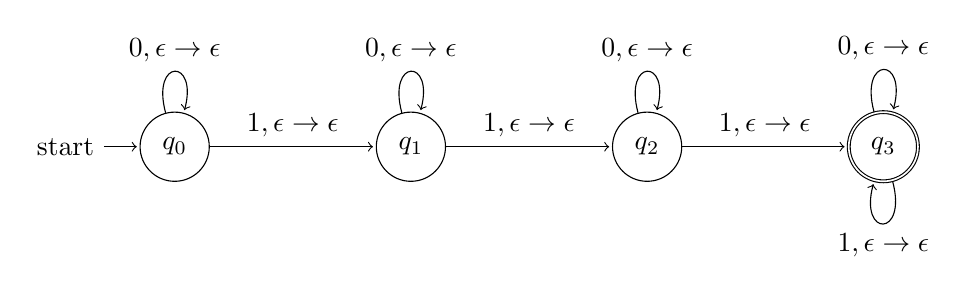
\begin{tikzpicture}[shorten >=1pt, node distance=3cm, on grid, auto]
    \node[state, initial] (q0) {$q_0$};
    \node[state] (q1) [right=of q0] {$q_1$};
    \node[state] (q2) [right=of q1] {$q_2$};
    \node[state, accepting] (q3) [right=of q2] {$q_3$};
    
    \path[->]
        (q0) edge[loop above] node {$0, \epsilon \to \epsilon$} ()
             edge node {$1, \epsilon \to \epsilon$} (q1)
        (q1) edge[loop above] node {$0, \epsilon \to \epsilon$} ()
             edge node {$1, \epsilon \to \epsilon$} (q2)
        (q2) edge[loop above] node {$0, \epsilon \to \epsilon$} ()
             edge node {$1, \epsilon \to \epsilon$} (q3)
        (q3) edge[loop above] node {$0, \epsilon \to \epsilon$} ()
             edge[loop below] node {$1, \epsilon \to \epsilon$} ();
\end{tikzpicture}

\subsection{b) Starts and ends with the same symbol}

This is a regular language. The PDA remembers the first symbol and checks at the end whether it matches.

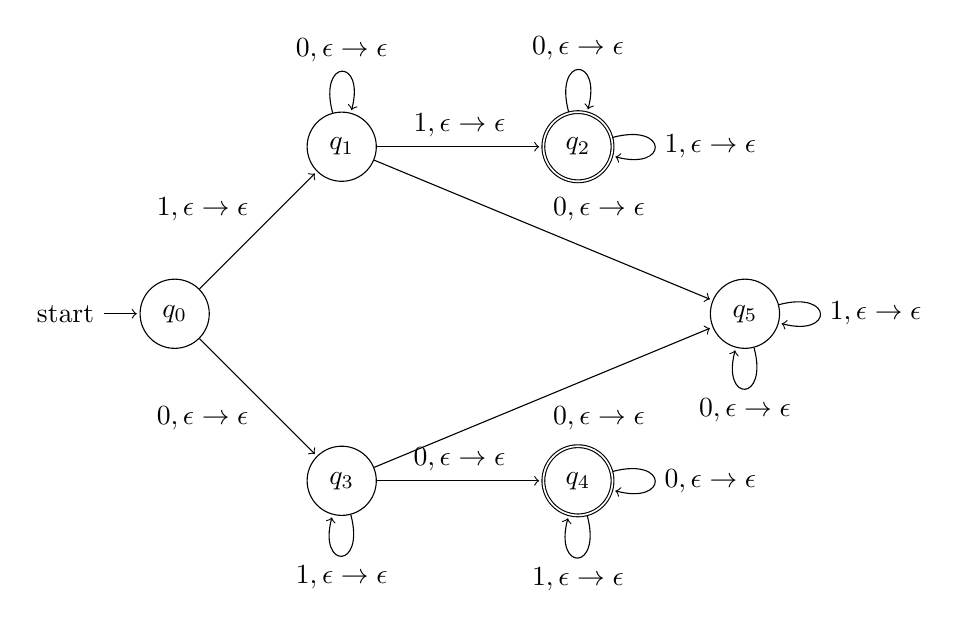
\begin{tikzpicture}[shorten >=1pt, node distance=3cm, on grid, auto]
    \node[state, initial] (q0) {$q_0$};
    \node[state] (q1) [above right=of q0] {$q_1$};
    \node[state, accepting] (q2) [right=of q1] {$q_2$};
    \node[state] (q3) [below right=of q0] {$q_3$};
    \node[state, accepting] (q4) [right=of q3] {$q_4$};
    \node[state] (q5) [below right=of q2] {$q_5$};
    
    \path[->]
        (q0) edge node {$1, \epsilon \to \epsilon$} (q1)
             edge node[swap] {$0, \epsilon \to \epsilon$} (q3)
        (q1) edge node {$1, \epsilon \to \epsilon$} (q2)
             edge[loop above] node {$0, \epsilon \to \epsilon$} ()
             edge node {$0, \epsilon \to \epsilon$} (q5)
        (q2) edge[loop above] node {$0, \epsilon \to \epsilon$} ()
             edge[loop right] node {$1, \epsilon \to \epsilon$} ()
        (q3) edge node {$0, \epsilon \to \epsilon$} (q4)
             edge[loop below] node {$1, \epsilon \to \epsilon$} ()
             edge node[swap] {$0, \epsilon \to \epsilon$} (q5)
        (q4) edge[loop right] node {$0, \epsilon \to \epsilon$} ()
             edge[loop below] node {$1, \epsilon \to \epsilon$} ()
        (q5) edge[loop below] node {$0, \epsilon \to \epsilon$} ()
             edge[loop right] node {$1, \epsilon \to \epsilon$} ();
\end{tikzpicture}

\subsection{c) Odd length}

This is a regular language. Two states alternate to represent even and odd length.

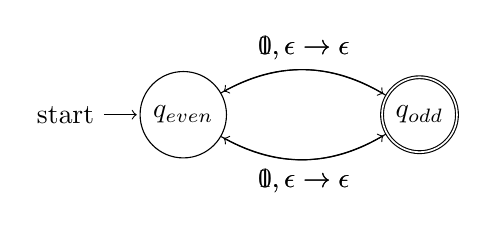
\begin{tikzpicture}[shorten >=1pt, node distance=3cm, on grid, auto]
    \node[state, initial] (q0) {$q_{even}$};
    \node[state, accepting] (q1) [right=of q0] {$q_{odd}$};
    
    \path[->]
        (q0) edge[bend left] node {$0, \epsilon \to \epsilon$} (q1)
             edge[bend right, swap] node {$1, \epsilon \to \epsilon$} (q1)
        (q1) edge[bend left] node {$0, \epsilon \to \epsilon$} (q0)
             edge[bend right, swap] node {$1, \epsilon \to \epsilon$} (q0);
\end{tikzpicture}

\subsection{d) Odd length with middle symbol 0}

This is a non-regular language. The PDA nondeterministically guesses the middle position: pushes the first half onto the stack, then matches the second half against the stack.

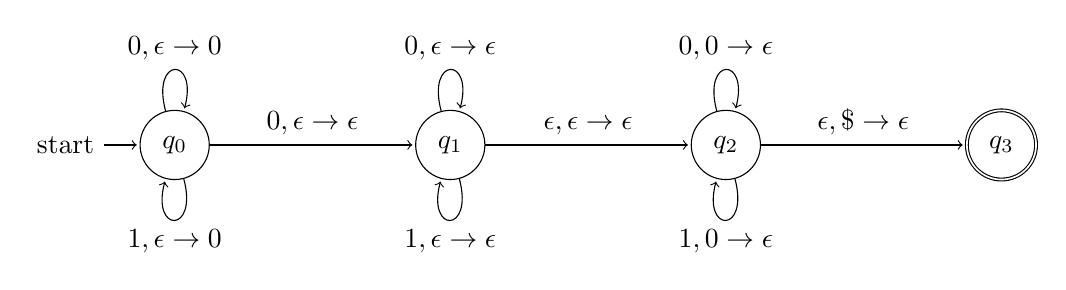
\begin{tikzpicture}[shorten >=1pt, node distance=3.5cm, on grid, auto]
    \node[state, initial] (q0) {$q_0$};
    \node[state] (q1) [right=of q0] {$q_1$};
    \node[state] (q2) [right=of q1] {$q_2$};
    \node[state, accepting] (q3) [right=of q2] {$q_3$};
    
    \path[->]
        (q0) edge[loop above] node {$0, \epsilon \to 0$} ()
             edge[loop below] node {$1, \epsilon \to 0$} ()
             edge node {$0, \epsilon \to \epsilon$} (q1)
        (q1) edge[loop above] node {$0, \epsilon \to \epsilon$} ()
             edge[loop below] node {$1, \epsilon \to \epsilon$} ()
             edge node {$\epsilon, \epsilon \to \epsilon$} (q2)
        (q2) edge[loop above] node {$0, 0 \to \epsilon$} ()
             edge[loop below] node {$1, 0 \to \epsilon$} ()
             edge node {$\epsilon, \$ \to \epsilon$} (q3);
\end{tikzpicture}

\begin{remark}
We use 0 as a symbol for counting.
\end{remark}

\subsection{e) Palindrome}

This is a non-regular language. Classic PDA: pushes the first half onto the stack, guesses the middle, and matches the second half.

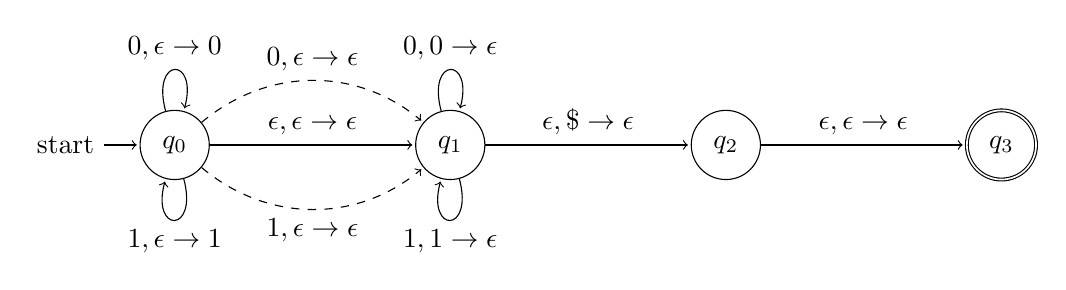
\begin{tikzpicture}[shorten >=1pt, node distance=3.5cm, on grid, auto]
    \node[state, initial] (q0) {$q_0$};
    \node[state] (q1) [right=of q0] {$q_1$};
    \node[state] (q2) [right=of q1] {$q_2$};
    \node[state, accepting] (q3) [right=of q2] {$q_3$};
    
    \path[->]
        (q0) edge[loop above] node {$0, \epsilon \to 0$} ()
             edge[loop below] node {$1, \epsilon \to 1$} ()
             edge node {$\epsilon, \epsilon \to \epsilon$} (q1)
        (q1) edge[loop above] node {$0, 0 \to \epsilon$} ()
             edge[loop below] node {$1, 1 \to \epsilon$} ()
             edge node {$\epsilon, \$ \to \epsilon$} (q2)
        (q2) edge node {$\epsilon, \epsilon \to \epsilon$} (q3);
        
    \path[->, dashed]
        (q0) edge[bend left=40] node[above] {$0, \epsilon \to \epsilon$} (q1)
             edge[bend right=40] node[below] {$1, \epsilon \to \epsilon$} (q1);
\end{tikzpicture}

\subsection{f) Empty set}

A PDA that accepts no strings: no accepting state, or no way to reach an accepting state.

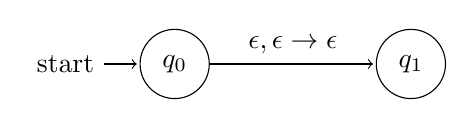
\begin{tikzpicture}[shorten >=1pt, node distance=3cm, on grid, auto]
    \node[state, initial] (q0) {$q_0$};
    \node[state] (q1) [right=of q0] {$q_1$};
    
    \path[->]
        (q0) edge node {$\epsilon, \epsilon \to \epsilon$} (q1);
\end{tikzpicture}

\section{Question 5} 

\subsection{a)} 

\begin{align*} 
S &\to SS \mid AaA \\
A &\to a A b \mid b A a \mid A A \mid \epsilon
\end{align*}

\subsection{b)}

\begin{align*} 
S &\to X b a X \mid C \mid D \\
X &\to a X \mid b X \mid \epsilon \\
C &\to a C b \mid a C \mid a \\
D &\to a D b \mid D b \mid b
\end{align*}

\section{Question 6} 

We first add a new start symbol: 

\begin{align*} 
A_0 &\to A \\ 
A &\to B A B \mid B \mid \epsilon \\
B &\to 11 \mid \epsilon 
\end{align*}

Then we eliminate $\epsilon$-productions:

\begin{align*} 
A_0 &\to A \mid \epsilon \\ 
A &\to B A B \mid BA \mid AB \mid BB \mid B\\
B &\to 11 
\end{align*}

We eliminate unit productions:

\begin{align*} 
A_0 &\to B A B \mid BA \mid AB \mid BB \mid 11 \mid \epsilon \\ 
A &\to B A B \mid BA \mid AB \mid BB \mid 11\\
B &\to 11 
\end{align*}

Finally, we convert to CNF (Chomsky Normal Form):

Let $C \to AB$, $D \to 1$, and we have 

\begin{align*} 
A_0 &\to BC \mid BA \mid AB \mid BB \mid DD \mid \epsilon \\ 
A &\to B C \mid BA \mid AB \mid BB \mid DD\\
C &\to AB \\
B &\to DD \\
D &\to 1 \\
\end{align*}

\end{document}